Mặc dù dữ liệu đã trải qua quá trình chuẩn hóa, khử nhiễu và vẫn giữ được các đặc trưng gốc, bước gán nhãn (data labeling) vẫn là công đoạn bắt buộc không thể bỏ qua. Theo cách làm truyền thống, công đoạn này đòi hỏi sự đánh giá độc lập từ ít nhất ba chuyên gia để đảm bảo độ chuẩn xác và tính trung lập; tuy nhiên, cách tiếp cận này tiêu tốn đáng kể nhân lực và ngân sách, đồng thời khó lòng mở rộng khi áp dụng cho những tập ngữ liệu lên đến hàng triệu mẫu.

Bởi vậy, xây dựng quy trình gán nhãn bán tự động (semi-automated labeling), kết hợp giữa sức mạnh tính toán của máy móc và tri thức chuyên gia, đang trở thành tất yếu. Những bước tiến vượt bậc của \acrlong{llm}, được áp dụng rộng rãi như một quy trình chuẩn trong nhiều dự án học thuật \parencite{hung2026vigoemotions, ding2026scope, wang2023self, ratner2017snorkel}.

\begin{figure}[htbp]
    \centering
    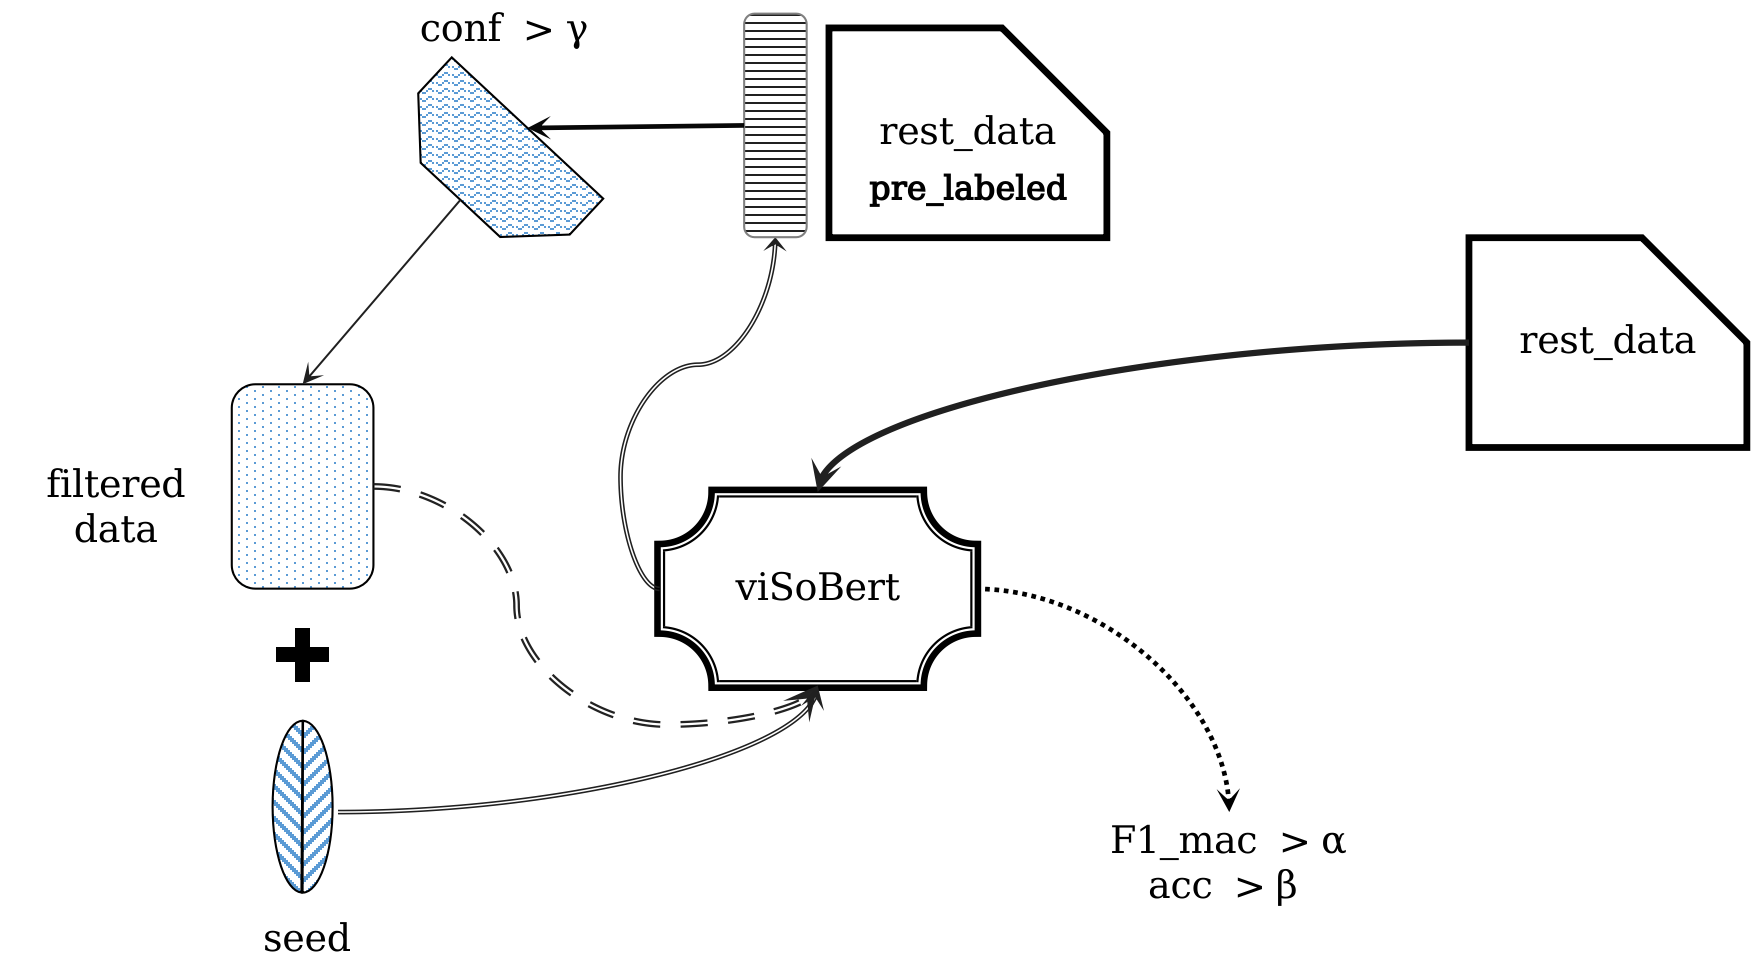
\includegraphics[width=0.85\textwidth]{Images/anno_proc.png}
    \caption{Quy trình gán nhãn bán tự động}
    \label{fig:gannhanbantudong}
    \vspace{0.1cm}
\end{figure}

Dựa trên cách tiếp cận của \textcite{ding2026scope}, quy trình gán nhãn bán tự động trong đề án được minh họa chi tiết qua Hình \ref{fig:gannhanbantudong}, với các bước như sau:

\textbf{Xây dựng tập hạt giống và cân bằng dữ liệu.}

Ban đầu, một tập dữ liệu hạt giống (seed dataset) gồm 10.000 mẫu được lấy theo xác suất đồng đều từ kho dữ liệu đã qua tiền xử lý. Để khắc phục tình trạng phân phối lệch ở các nhãn hiếm gặp (như "\texttt{grief}", "\texttt{nervousness}", "\texttt{remorse}", \dots), một phương pháp trích xuất dựa trên tập luật từ vựng (rule-based) được tích hợp thêm nhằm bổ sung mẫu. Cụ thể:

\begin{itemize}[label=-]
    \item Những văn bản chứa các từ khóa như \textit{"chia buồn"}, \textit{"xót xa"}, \textit{"mất mát"}, \textit{"vĩnh biệt"} hay \textit{"rip"} có khả năng cao thuộc về nhãn \texttt{grief}.
    \item Tương tự, các từ khóa \textit{"xin lỗi"}, \textit{"hối hận"}, \textit{"cắn rứt"} được dùng để lọc ra những mẫu khả năng cao thuộc nhãn \texttt{remorse}.
\end{itemize}

Tiếp đó, tập hạt giống được mở rộng thêm dữ liệu từ bộ ngữ liệu \textbf{ViGoEmotions} nhằm gia tăng độ phong phú cả về quy mô lẫn chiều sâu ngữ nghĩa. Bên cạnh đó, do độ chênh lệch phân bố lớn (khoảng 1:30) giữa nhãn hiếm và nhãn phổ biến, kỹ thuật sinh dữ liệu nhân tạo (synthetic data generation) thông qua các mô hình LLMs (như Gemini, GPT, \dots) áp dụng làm giàu thêm tập dữ liệu huấn luyện.

\textbf{Thiết lập mô hình nền tảng.}

Khi hoàn tất tập hạt giống, đề án lựa chọn một hệ thống xử lý ngôn ngữ tự nhiên từ kiến trúc Encoder. Cụ thể là ViSoBert \parencite{nguyen2023visobert}, mô hình đã huấn luyện (pre-trained) trên ngữ liệu mạng xã hội Việt Nam để đảm nhiệm nhiệm vụ gán nhãn.

\textbf{Vòng lặp gán nhãn giả (Iterative Pseudo-labeling)}

Vòng lặp (iteration) của hệ thống gán nhãn khởi động bằng việc tinh chỉnh (fine-tuning) mô hình trên tập hạt giống nhằm tối đa hóa năng lực phân loại, với mục tiêu trọng tâm là cực đại hóa chỉ số F1-macro. Phiên bản mô hình sau tinh chỉnh này sau đó đảm nhận vai trò gán nhãn tự động (gán nhãn giả - pseudo labeling) cho toàn bộ phần ngữ liệu thô còn lại.

Căn cứ vào kết quả dự đoán, các mẫu dữ liệu mới được trích xuất và cập nhật vào tập huấn luyện cho vòng lặp kế tiếp, theo chiến lược chọn mẫu động:

\begin{itemize}[label=-]
    \item \textbf{Giai đoạn đầu (khi tập mồi < 100.000 mẫu hoặc phân bố nhãn chưa đồng đều)}: thuật toán trích xuất \texttt{K\_SAMPLE} mẫu có độ tin cậy dự đoán (prediction probability) cao nhất ứng với mỗi nhãn để bổ sung cho tập huấn luyện mới.
    \item \textbf{Giai đoạn sau (khi tập huấn luyện đã đạt kích thước đủ lớn)}: chỉ những mẫu có xác suất dự đoán vượt một ngưỡng tin cậy cố định (ví dụ: $> 0.85$ hoặc $> 0.9$) mới tiếp tục được trích xuất.
\end{itemize}

